\newcommand{\vocab}{\mathbf{v}}
\newcommand{\dtvec}{\mathbf{t}_\Delta}
\newcommand{\ctxvec}{\mathbf{t}_\text{ctx}}
\newcommand{\dt}{\Delta_t}
\newcommand{\prerror}{Pr_{error}}
\newcommand{\weights}{\mathbf{w}}
\newcommand{\X}{\mathbf{X}}
\newcommand{\post}{\rho}
\renewcommand{\t}{t}
\newcommand{\w}{w}
Our project aims to predict the amount of time between the arrival of the next 
post and the time the last post in the thread was made. The information 
available to us are the previously made posts that we observe when first 
visiting the thread. The assumption made here is that the thread is not 
paginated in any way, and a single visit to the thread gives us the latest posts 
without having to traverse through the links to the latest page.

More formally, what we are trying to do is to estimate a function $f$ such that 
given a feature vector $\X$ representative of a window $\post_{t - w + 
1},\post_{t - w + 2},\cdots ,\post_t$, we can approximate $\dt$ with $f(\X)$. In 
the following sections, we will discuss various methods for estimating $f$.  
Various notations will be used, a quick reference is provided in Table 
\ref{table:notations}.

\begin{table}
	\begin{center}
	\begin{tabular}{l l}
	\hline
Notation	&	Description\\
	\hline
$\post$		&	A post\\
$\t$		&	Index of a post in a thread\\
$\w$		&	Number of posts in a window\\
$\post_\t$	&	The $t$-th post in the thread\\
$\vocab_\t$	&	The frequency count vector of the posts used in the $t$-th 
	post\\
$\dt$		&	Time difference between a post at position $\t$ and a post at 
	position $\t+1$ \\
$\dtvec$	&	Vector of $\dt$s in a given window\\
$\ctxvec$	&	Bit vector representing the day of week, and the hour of day\\
$\X$		&	Feature vector extracted from a window\\
	\hline
	\end{tabular}
\end{center}
\caption{Notation reference} \label{table:notations}
\end{table}


We extracted the timestamp, author and text content for each post in each thread
from the forums. Our dataset was obtained from from \url{avsforums.com}.
%
%\begin{description}
%	\item[Previous time differences] All the time differences between posts made 
%		in the window. ($\dtvec$)
%	\item[Time-based features] Day of week, Hour of day. Provides contextual 
%		information about when the post was made. ($\ctxvec$)
%	\item[Content features (text)] Word frequency counts are used for this set 
%		of experiments. Using regression, we find the top $K$ variables that the 
%		actual $\dt$ depends on.  Table \ref{vocab_exp} reflect the results of 
%		the experiments done with varying values of $K$.
%\end{description}
%

\section{Baselines}
A simple way of estimating the revisit rate would be to use the average time 
differences given the observed posts, or a training set. In previous work, we 
have seen that if page updates follow a Poisson distribution, then revisiting at 
the Poisson mean would be an optimal revisit policy. %cite paper.

There are some details that need to be considered. One revisit policy would be 
to do so at a constant, fixed rate, independent of the posts being made to the 
thread. For our baseline revisit policy, we took into account the last made post 
whenever we revisit, and calculate our next revisit time based on the last post.

Another way of predicting using average post interval timings would be to use a 
sliding window. Averaging out the time differences between the posts would 
intuitively work, because it captures the context of the situation: A series of 
posts with short intervals should mean that the next post would come at around 
the same interval as the few that came before.


\begin{figure}
	\begin{center}
	
\tikzstyle{background}=[rectangle,
	fill=gray!10,
	inner sep=0.2cm,
	rounded corners=5mm]


\tikzstyle{post}=[circle,
	thick,
	minimum size=1.2cm,
	draw=blue!80,
	fill=blue!20]
% The measurement vector is represented by an orange circle.
\tikzstyle{visit}=[circle,
	thick,
	minimum size=1.2cm,
	draw=orange!80,
	fill=orange!25]

\begin{tikzpicture}[>=latex,text height=1.5ex,text depth=0.25ex]
    % "text height" and "text depth" are required to vertically
    % align the labels with and without indices.
  
  % The various elements are conveniently placed using a matrix:
  \matrix[column sep=0.3cm] {
    % First line: Control input
    	&
		\node (e0)					{};&
		\node (e1)	[post]			{};&
		\node (e2)	[visit]			{};&
		\node (e3)	[post]			{};&
		\node (e4)	[visit]			{};&
		\node (e5)	[post]			{};&
		\node (e6)	[visit]			{};&
		\node (e)					{};&
		&
        \\
	};
    
    % The diagram elements are now connected through arrows:

	\path[-]
		(e0) edge[thick]	(e1)
		\foreach \e in {1,2,3,4,5}{
			let \n1={int(\e+1)} in (e\e) edge[thick] (e\n1)
		}
		(e6) edge[thick]	(e)
	;

	\begin{pgfonlayer}{background}
		\node [background,fit=(e1) (e3)] {};
	\end{pgfonlayer}

\end{tikzpicture}


\begin{tikzpicture}[>=latex,text height=1.5ex,text depth=0.25ex]
    % "text height" and "text depth" are required to vertically
    % align the labels with and without indices.
  
  % The various elements are conveniently placed using a matrix:
  \matrix[column sep=0.3cm] {
    % First line: Control input
    	&
		\node (e0)					{};&
		\node (e1)	[post]			{}; &
		\node (e2)	[visit]			{}; &
		\node (e3)	[post]			{}; &
		\node (e4)	[visit]			{}; &
		\node (e5)	[post]			{}; &
		\node (e6)	[visit]			{}; &
		\node (e)					{};&
		&
        \\
	};
    
    % The diagram elements are now connected through arrows:

	\path[-]
		(e0) edge[thick]	(e1)
		\foreach \e in {1,2,3,4,5}{
			let \n1={int(\e+1)} in (e\e) edge[thick] (e\n1)
		}
		(e6) edge[thick]	(e)
	;

	\begin{pgfonlayer}{background}
		\node [background,fit=(e3) (e5)] {};
	\end{pgfonlayer}

\end{tikzpicture}

	\caption{%
A series of events, posts (blue) and visits (orange).  The diagram demonstrates 
the concept of a window of $w=2$.
}\label{fig:event_series}
	\end{center}
\end{figure}

We will also be using figures similar to those found in Figure 
\ref{fig:event_series}. In these diagrams, blue nodes represent post events and 
orange nodes represent visit events.


\section{Performing regression on windows}
Previous work has used linear regression on a number of different features 
extracted from forums \cite{Yang2009}. In their paper, the regressed function 
was used as a scoring function rather than a predictive function. In site of 
this, we attempted to implement the same model, but this resulted in evaluations 
worse than that of the baseline.

We did use some of the features mentioned in the paper: Window posts time 
differences and time context features (bit-vector representations of the day of 
the week and hour of the day). In our own statistics we took from the 
\url{avsforum.com} threads, we have also found that the time of the day the day 
of the week matters when dealing with threads. An example of such a thread can 
be seen in Figure \ref{fig:hr_freq} and Figure \ref{fig:week_freq}, where it can 
be seen that activity on the board is highest at 2 PM, and drops slightly, 
suggesting some type of lunch period, and then goes up again during the early 
evening and at 9 PM, before dropping to its lowest at 3 AM. The weekly graph 
also shows a pattern, showing lower posting frequencies during the weekends, and 
its highest during Thursdays.

\begin{figure}
\begin{center}
\begin{subfigure}[b]{0.8\textwidth}
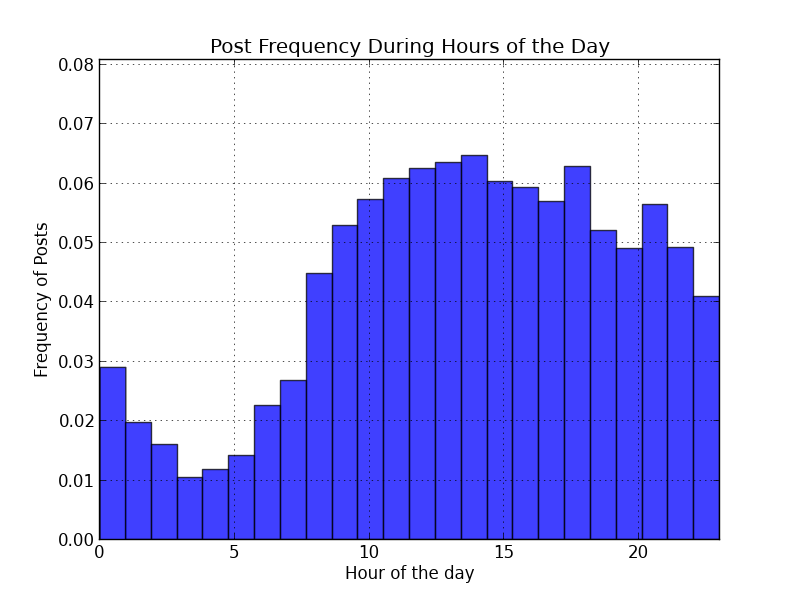
\includegraphics[width=\textwidth]{diagrams/hoursofday.png}
\caption{The hourly post frequency for the hours during the day.}
\label{fig:hr_freq}
	\end{subfigure}
	\begin{subfigure}[b]{0.8\textwidth}
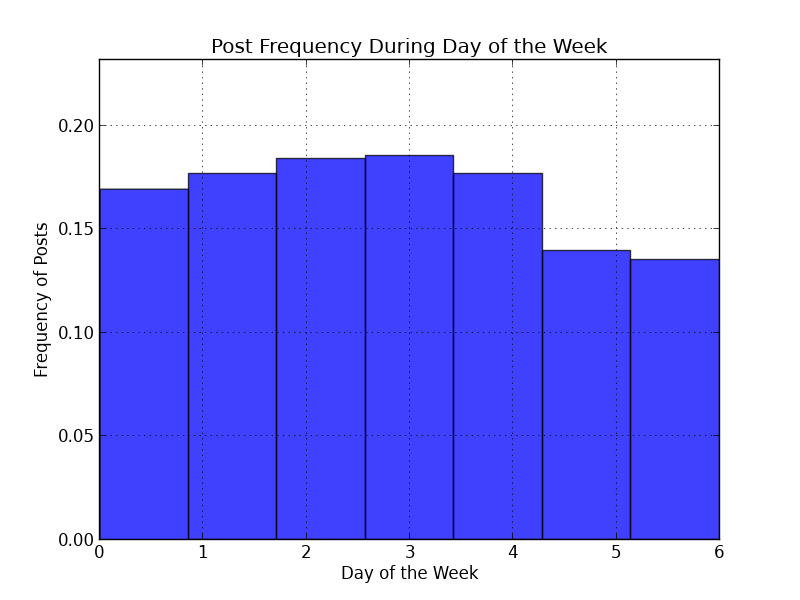
\includegraphics[width=\textwidth]{diagrams/daysofweek.png}
\caption{The daily post frequency for the hours during the week. (Monday is 0)}
\label{fig:week_freq}
	\end{subfigure}
\end{center}
\end{figure}

However, this time in stead of linear regression, we used a regression method 
known as Support Vector Regression (SVR). This method allows the using of 
different kernels, allowing for better estimation of the target function.

The main focus of study in this report was to see if content helps with 
predicting thread updates would produce an improvement. Some of the ways that 
content data were extracted into feature vectors are the following: Word 
frequency, the tf-idf of these words, and Part-of-Speech tags.

We perform the standard preprocessing steps like removing stopwords and tokens 
of length less than three. We also use Porter's stemming algorithm as another 
preprocessing step, before performing a word frequency count. However, the use 
of the full vocabulary of the thread as a feature vector greatly increases the 
time needed to train the model. As such, we used a simple univariate regression 
technique for feature selection, and selected only the $K$ best tokens for 
consideration. Table \ref{table:vocab_exp} shows the results of this experiment.  

\begin{table}
	\footnotesize
	\begin{centering}
	\begin{tabular}{|l|c|c|c|c|c|c|c|c|}
	\hline
	\input{tables/vocab_exp}
	\hline
	\end{tabular}
	\caption{Experiment results: Varying vocabulary size}
	\label{table:vocab_exp}
\end{centering}
\end{table}


These feature sets are used in different combinations, with different window 
sizes. The results will be seen in the next chapter.

\section{Discounted sum of previous instances}
The current method uses only information on the current $w$ posts. However, 
posts made further in the history of the thread may have an effect on when the 
latest posts arrive. The magnitude of this effect, however, may diminish over 
time.

Following this intuition we attempt to use a discounted sum over previous posts' 
word frequency vector:
\[
	\X'_t = \X_t + \alpha \X'_{t-1}
\]
where $\X_t$ is the feature vector at post $t$, and $\vocab$ is the word 
frequency vector. $\alpha$ is the \emph{discount factor} and satisfies $0 \leq 
\alpha < 1$.

\section{Stochastic Gradient Descent}

We attempt to use stochastic gradient descent to estimate the function $f$.  
However, during runtime, instead of using a static function, we continue to 
allow $f$ to vary whenever new posts and their update times are observed.
Since $f(\X_{t-w},\hdots,\X_{t-1}) > 0$, we used a scaled sigmoid function,
\[
	f(\X) = \frac{\Lambda-\lambda}{1 + e^{\weights \cdot \X}} + \lambda
\]
where $\Lambda$ and $\lambda$ are the scaling factors. This results in $f: 
\mathbb{R}^{|\X|}  \rightarrow (\lambda,\Lambda)$. Bounding the estimation 
function between $\lambda$ and $\Lambda$ allows us to restrict the prediction 
from becoming negative, or, becoming exceedingly huge. For our purposes, we set 
$\lambda = Q_3 + 2.5(Q_{3} - Q_{1})$, where $Q_n$ is the value at the $n$-th 
quartile. 

The resulting update rule for $\weights$ is then given by,
\[
	\Delta \weights_i = \eta
				\underbrace{\left(\widehat{\dt} - \dt \right)}_{\text{error term}}
				\underbrace{\left( f(\X)(1-f(\X)) \right)}_{\text{gradient}}
						\X_i
\]
which is similar to the delta update rule found in artificial neural networks.  
We omit the scaling factor in the gradient as it is a constant and then 
experiment with various values of $\eta$, the learning rate. 

